\باب{سوالات امالہ، برق گیر}
%============================
\ابتدا{سوال}
ایک سو مائیکرو فیراڈ کے برق گیر میں دس سیکنڈ کے لئے  ایک ملی ایمپیئر رو سے بار بھرنے کے بعد برق گیر کا دباو دریافت کریں۔

جواب:\عددی{\SI{100}{\volt}}  
\انتہا{سوال}
%========================
\ابتدا{سوال}
\عددی{\SI{8}{\micro\farad}} کے برق گیر پر \عددی{\SI{4}{\milli\coulomb}} بار پایا جاتا ہے۔اس پر دباو دریافت کریں۔

جواب:\عددی{\SI{500}{\volt}}
\انتہا{سوال}
%=======================
\ابتدا{سوال}
ایک برق گیر پر \عددی{\SI{12}{\volt}} دباو اور \عددی{\SI{96}{\nano\farad}}  بار پایا جاتا ہے۔اس کی گنجائش دریافت کریں۔

جواب:\عددی{C=\SI{8}{\nano\farad}}
\انتہا{سوال}
%=====================
\ابتدا{سوال}
ایک برق گیر پر ابتدائی دباو \عددی{\SI{-20}{\volt}} ہے جبکہ اس کی گنجائش \عددی{C=\SI{5}{\micro\farad}} ہے۔اس میں \عددی{\SI{2}{\micro\ampere}} سے \عددی{\SI{90}{\second}} کے لئے بار بھرا جاتا ہے۔برق گیر پر اختتامی دباو حاصل کریں۔

جواب:\عددی{\SI{16}{\volt}}
\انتہا{سوال}
%=====================
\ابتدا{سوال}
\عددی{\SI{12}{\micro\farad}} برق گیر میں ذخیرہ توانائی \عددی{6\cos^2 3000t \, \si{\micro\joule}} ہے۔برق گیر کی رو دریافت کریں۔ 

جواب:\عددی{i_C=-0.036\sin 3000t \,\si{\ampere}}
\انتہا{سوال}
%====================
\ابتدا{سوال}\شناخت{سوال_برق_گیر_رو_دباو_الف}
ابتدائی طور پر بے بار \عددی{\SI{0.2}{\milli\farad}} برق گیر کو شکل \حوالہ{شکل_سوال_برق_گیر_رو_دباو_الف} کی رو سے بھرا جاتا ہے۔برق گیر پر دباو کا خط کھینچیں۔
\begin{figure}
\centering
\begin{subfigure}{0.5\textwidth}
\centering
\begin{tikzpicture}
\begin{axis}[small,xlabel={$t\,(\si{\second})$},ylabel={$i,\,(\si{\milli\ampere})$},xtick={0,3,4,6},xticklabels={$0$,$3$,$4$,$6$},ytick={0,1,2},yticklabels={$0$,$10$,$20$},ylabel style={rotate=-90},ylabel style={at={(axis description cs:0,1.05)}}]
\addplot[] plot coordinates {(-0.5,0) (0,0) (0,1) (3,1) (3,0) (4,0) (4,2) (6,2) (6,0)(6.5,0) };
\end{axis}
\end{tikzpicture}
\caption*{(الف)}
\end{subfigure}%
\begin{subfigure}{0.5\textwidth}
\centering
\begin{tikzpicture}
\begin{axis}[small,xlabel={$t\,(\si{\second})$},ylabel={$v_C,\,(\si{\volt})$},xtick={0,3,4,6},xticklabels={$0$,$3$,$4$,$6$},ytick={0,150,350},yticklabels={$0$,$150$,$350$},ylabel style={rotate=-90},ylabel style={at={(axis description cs:0,1.05)}}]
\addplot[] plot coordinates {(-0.5,0) (0,0)  (3,150) (4,150)  (6,350) (6.5,350) };
\end{axis}
\end{tikzpicture}
\caption*{(ب)}
\end{subfigure}%
\caption{سوال \حوالہ{سوال_برق_گیر_رو_دباو_الف} کے اشکال۔}
\label{شکل_سوال_برق_گیر_رو_دباو_الف}
\end{figure}

جواب:شکل-ب میں دباو دکھایا گیا ہے۔
\انتہا{سوال}
%=====================
\ابتدا{سوال}\شناخت{سوال_برق_گیر_رو_دباو_ب}
  \عددی{\SI{10}{\micro\farad}} برق گیر کے دباو کو شکل \حوالہ{شکل_سوال_برق_گیر_رو_دباو_ب} میں دکھایا گیا ہے۔اس کی رو کا خط کھینچیں۔
\begin{figure}
\centering
\begin{subfigure}{0.5\textwidth}
\centering
\begin{tikzpicture}
\begin{axis}[small,xlabel={$t\,(\si{\milli\second})$},ylabel={$v_C,\,(\si{\volt})$},xtick={0,4,6,8},xticklabels={$0$,$4$,$6$,$8$},ytick={0,100},yticklabels={$0$,$100$},ylabel style={rotate=-90},ylabel style={at={(axis description cs:0,1.05)}}]
\addplot[] plot coordinates {(-0.5,0) (0,0) (4,100) (6,100) (8,0) (8.5,0)};
\end{axis}
\end{tikzpicture}
\caption*{(الف)}
\end{subfigure}%
\begin{subfigure}{0.5\textwidth}
\centering
\begin{tikzpicture}
\begin{axis}[small,xlabel={$t\,(\si{\milli\second})$},ylabel={$i_C,\,(\si{\milli\ampere})$},xtick={0,4,6,8},xticklabels={$0$,$4$,$6$,$8$},ytick={0,250,-500},yticklabels={$0$,$250$,$-500$},ylabel style={rotate=-90},ylabel style={at={(axis description cs:0,1.05)}}]
\addplot[] plot coordinates {(-0.5,0) (0,0) (0,250) (4,250) (4,0) (6,0) (6,-500) (8,-500) (8,0) (8.5,0)};
\end{axis}
\end{tikzpicture}
\caption*{(ب)}
\end{subfigure}%
\caption{سوال \حوالہ{سوال_برق_گیر_رو_دباو_ب} کے اشکال۔}
\label{شکل_سوال_برق_گیر_رو_دباو_ب}
\end{figure}

جواب:شکل-ب میں رو دکھائی گئی ہے۔
\انتہا{سوال}
%=====================
\ابتدا{سوال}\شناخت{سوال_برق_گیر_رو_دباو_پ}
  \عددی{\SI{0.4}{\farad}} برق گیر کی رو کو شکل \حوالہ{شکل_سوال_برق_گیر_رو_دباو_پ} میں دکھایا گیا ہے۔اس پر دباو کا خط کھینچیں۔
\begin{figure}
\centering
\begin{subfigure}{0.5\textwidth}
\centering
\begin{tikzpicture}
\begin{axis}[small,xlabel={$t\,(\si{\second})$},ylabel={$i_C,\,(\si{\ampere})$},xtick={0,5,7,10},xticklabels={$0$,$5$,$7$,$10$},ytick={0,12,40},yticklabels={$0$,$12$,$40$},ylabel style={rotate=-90},ylabel style={at={(axis description cs:0,1.05)}}]
\addplot[] plot coordinates {(-0.5,0) (0,0) (5,40) (5,0)(7,0) (7,12) (10,12) (10,0) (11,0)};
\end{axis}
\end{tikzpicture}
\caption*{(الف)}
\end{subfigure}%
\begin{subfigure}{0.5\textwidth}
\centering
\begin{tikzpicture}
\begin{axis}[small,xlabel={$t\,(\si{\second})$},ylabel={$v_C,\,(\si{\volt})$},xtick={0,5,7,10},xticklabels={$0$,$5$,$7$,$10$},ytick={0,250,340},yticklabels={$0$,$250$,$340$},ylabel style={rotate=-90},ylabel style={at={(axis description cs:0,1.05)}}]
\addplot[] plot coordinates {(-0.5,0)(0,0)};
\addplot[domain=0:5]{10*x^2};
\addplot[]plot coordinates {(5,250) (7,250) (10,340) (11,340)}; 
\end{axis}
\end{tikzpicture}
\caption*{(ب)}
\end{subfigure}%
\caption{سوال \حوالہ{سوال_برق_گیر_رو_دباو_پ} کے اشکال۔}
\label{شکل_سوال_برق_گیر_رو_دباو_پ}
\end{figure}

جواب:شکل-ب میں دباو دکھایا گیا ہے۔
\انتہا{سوال}
%=====================
\ابتدا{سوال}\شناخت{سوال_برق_گیر_رو_دباو_ت}
 \عددی{\SI{0.1}{\farad}} برق گیر کا دباو شکل \حوالہ{شکل_سوال_برق_گیر_رو_دباو_ت} میں دیا گیا ہے۔اس کی رو کا خط کھینچیں۔
\begin{figure}
\centering
\begin{subfigure}{0.5\textwidth}
\centering
\begin{tikzpicture}
\begin{axis}[small,xlabel={$t\,(\si{\second})$},ylabel={$v_C,\,(\si{\volt})$},ylabel style={rotate=-90},ylabel style={at={(axis description cs:0,1.05)}},xtick={2.5,5,7.5,10},xticklabels={$2.5$,$5$,$7.5$,$10$},ytick={-1,0,1},yticklabels={$-1$,$0$,$1$}]
\addplot[domain=0:10,smooth] {sin(36*x)}; 
\end{axis}
\end{tikzpicture}
\caption*{(الف)}
\end{subfigure}%
\begin{subfigure}{0.5\textwidth}
\centering
\begin{tikzpicture}
\begin{axis}[small,xlabel={$t\,(\si{\second})$},ylabel={$i_C,\,(\si{\ampere})$},ylabel style={rotate=-90},ylabel style={at={(axis description cs:0,1.05)}},xtick={2.5,5,7.5,10},xticklabels={$2.5$,$5$,$7.5$,$10$},ytick={-3.6,0,3.6},yticklabels={$-3.6$,$0$,$3.6$}]
\addplot[domain=0:10,smooth] {3.6*cos(36*x)}; 
\end{axis}
\end{tikzpicture}
\caption*{(ب)}
\end{subfigure}%
\caption{سوال \حوالہ{سوال_برق_گیر_رو_دباو_ت} کے اشکال۔}
\label{شکل_سوال_برق_گیر_رو_دباو_ت}
\end{figure}

جواب:شکل-ب میں رو دکھائی گئی ہے۔
\انتہا{سوال}
%=====================
\ابتدا{سوال}\شناخت{سوال_برق_گیر_رو_دباو_ٹ}
ابتدائی طور پر بے بار \عددی{\SI{10}{\micro\farad}} برق گیر کی رو شکل \حوالہ{شکل_سوال_برق_گیر_رو_دباو_ٹ} میں دی گئی ہے۔اس کے دباو کا خط کھینچیں۔
\begin{figure}
\centering
\begin{subfigure}{0.5\textwidth}
\centering
\begin{tikzpicture}
\begin{axis}[small,xlabel={$t\,(\si{\milli\second})$},ylabel={$i_C,\,(\si{\milli\ampere})$},ylabel style={rotate=-90},ylabel style={at={(axis description cs:0,1.05)}},xtick={10,20,30,40},xticklabels={$10$,$20$,$30$,$40$},ytick={-20,0,20},yticklabels={$-20$,$0$,$20$}]
\addplot[] plot coordinates {(-5,0) (0,0) (0,20) (10,20) (10,-20) (20,-20) (20,20) (30,20) (30,-20) (40,-20) (40,0) (45,0)}; 
\end{axis}
\end{tikzpicture}
\caption*{(الف)}
\end{subfigure}%
\begin{subfigure}{0.5\textwidth}
\centering
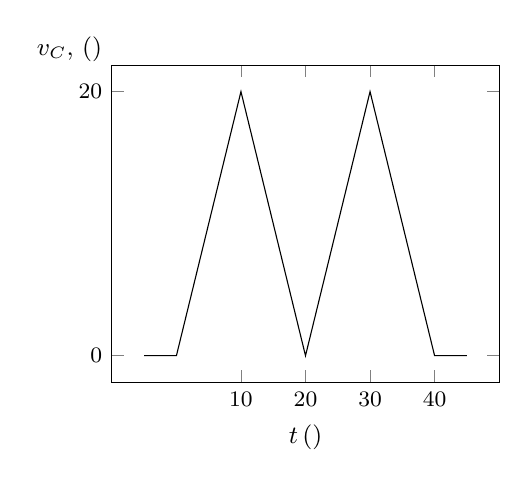
\begin{tikzpicture}
\begin{axis}[small,xlabel={$t\,(\si{\milli\second})$},ylabel={$v_C,\,(\si{\volt})$},ylabel style={rotate=-90},ylabel style={at={(axis description cs:0,1.05)}},xtick={10,20,30,40},xticklabels={$10$,$20$,$30$,$40$},ytick={0,20},yticklabels={$0$,$20$}]
\addplot[] plot coordinates {(-5,0) (0,0) (10,20) (20,0) (30,20) (40,0) (45,0)};
\end{axis}
\end{tikzpicture}
\caption*{(ب)}
\end{subfigure}%
\caption{سوال \حوالہ{سوال_برق_گیر_رو_دباو_ٹ} کے اشکال۔}
\label{شکل_سوال_برق_گیر_رو_دباو_ٹ}
\end{figure}

جواب:شکل-ب میں دباو دکھایا گیا ہے۔
\انتہا{سوال}
%=====================
\ابتدا{سوال}
ایک امالہ گیر میں \عددی{\SI{5}{\milli\second}} کے دورانیے میں رو \عددی{\SI{0}{\milli\ampere}} سے بڑھ کر \عددی{\SI{100}{\milli\ampere}} ہو جاتی ہے۔اس دورانیے میں امالی دباو \عددی{\SI{400}{\milli\volt}} ہوتا ہے۔امالہ گیر کی گنجائش دریافت کریں۔

جواب:\عددی{\SI{2}{\milli\henry}}
\انتہا{سوال}
%=============================
\ابتدا{سوال}
\عددی{\SI{50}{\milli\henry}} امالہ گیر کی رو \عددی{i=7\sin 314 t \, \si{\ampere}} ہے۔اس کے دباو کی مساوات حاصل کریں۔امالہ گیر میں ذخیرہ توانائی کی مساوات حاصل کریں۔

جواب:\عددی{v_L=109.9\cos 314t \,\si{\volt}}، \عددی{w=\tfrac{49}{40}\sin^2 314t \,\si{\joule}}
\انتہا{سوال}
%==========================
\ابتدا{سوال}
\عددی{\SI{0.4}{\henry}} امالہ گیر کی رو درج ذیل ہے۔لمحہ \عددی{t=\SI{-3}{\second}} اور \عددی{t=\SI{0.5}{\second}} پر امالہ کی رو اور امالہ میں ذخیرہ توانائی دریافت کریں۔
\begin{align*}
i_L=
\begin{cases}
0 & t<0\\
50(1-e^{-2t})\,\si{\milli\ampere} & t>0
\end{cases}
\end{align*}

جوابات:\عددی{\SI{0}{\ampere}}، \عددی{\SI{0}{\joule}}، \عددی{\SI{31.61}{\milli\ampere}}، \عددی{\SI{199.8}{\micro\joule}}
\انتہا{سوال}
%=========================
\ابتدا{سوال}\شناخت{سوال_امالہ_دباو_رو_خط_الف}
شکل \حوالہ{شکل_سوال_امالہ_دباو_رو_خط_الف} میں \عددی{\SI{3}{\henry}} کا دباو دیا گیا ہے۔اس کی رو کا خط کھینچیں۔ابتدائی رو صفر ہے۔
\begin{figure}
\centering
\begin{subfigure}{0.5\textwidth}
\centering
\begin{tikzpicture}
\begin{axis}[small,xlabel={$t\,(\si{\second})$},ylabel={$v,\,(\si{\volt})$},ylabel style={rotate=-90},ylabel style={at={(axis description cs:0,1.05)}},xtick={0,2,3,5},xticklabels={$0$,$2$,$3$,$5$},ytick={-10,0,10},yticklabels={$-12$,$0$,$12$}]
\addplot[] plot coordinates {(-0.5,0) (0,0) (0,12) (2,12) (2,0) (3,0) (3,-12) (5,-12) (5,0) (5.5,0) }; 
\end{axis}
\end{tikzpicture}
\caption*{(الف)}
\end{subfigure}%
\begin{subfigure}{0.5\textwidth}
\centering
\begin{tikzpicture}
\begin{axis}[small,xlabel={$t\,(\si{\second})$},ylabel={$i,\,(\si{\ampere})$},ylabel style={rotate=-90},ylabel style={at={(axis description cs:0,1.05)}},xtick={0,2,3,5},xticklabels={$0$,$2$,$3$,$5$},ytick={0,8},yticklabels={$0$,$8$}]
\addplot[] plot coordinates {(-0.5,0) (0,0)(2,8) (3,8) (5,0) (5.5,0) }; 
\end{axis}
\end{tikzpicture}
\caption*{(ب)}
\end{subfigure}%
\caption{سوال \حوالہ{سوال_امالہ_دباو_رو_خط_الف} کے اشکال۔}
\label{شکل_سوال_امالہ_دباو_رو_خط_الف}
\end{figure}

جواب:شکل-ب میں رو دی گئی ہے۔
\انتہا{سوال}
%=====================
\ابتدا{سوال}\شناخت{سوال_امالہ_دباو_رو_خط_ب}
شکل \حوالہ{شکل_سوال_امالہ_دباو_رو_خط_ب} میں \عددی{\SI{10}{\milli\henry}} کا دباو دیا گیا ہے۔اس کی رو کا خط کھینچیں۔ابتدائی رو صفر ہے۔
\begin{figure}
\centering
\begin{subfigure}{0.5\textwidth}
\centering
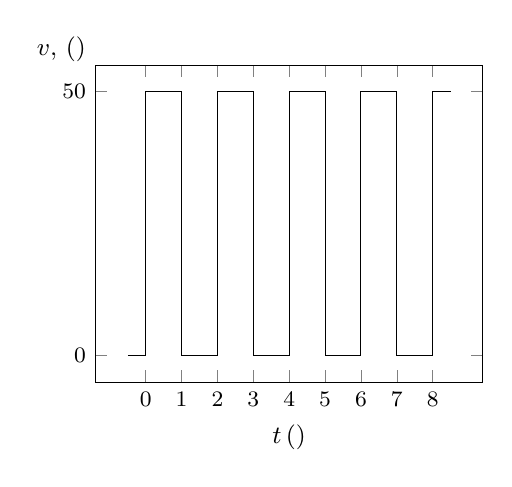
\begin{tikzpicture}
\begin{axis}[small,xlabel={$t\,(\si{\milli\second})$},ylabel={$v,\,(\si{\milli\volt})$},ylabel style={rotate=-90},ylabel style={at={(axis description cs:0,1.05)}},xtick={0,1,2,3,4,5,6,7,8},xticklabels={$0$,$1$,$2$,$3$,$4$,$5$,$6$,$7$,$8$},ytick={0,1},yticklabels={$0$,$50$}]
\addplot[] plot coordinates {(-0.5,0) (0,0) (0,1) (1,1) (1,0) (2,0) (2,1) (3,1) (3,0) (4,0) (4,1) (5,1) (5,0) (6,0) (6,1) (7,1) (7 ,0) (8,0) (8,1) (8.5,1) }; 
\end{axis}
\end{tikzpicture}
\caption*{(الف)}
\end{subfigure}%
\begin{subfigure}{0.5\textwidth}
\centering
\begin{tikzpicture}
\begin{axis}[small,xlabel={$t\,(\si{\milli\second})$},ylabel={$i,\,(\si{\milli\ampere})$},ylabel style={rotate=-90},ylabel style={at={(axis description cs:0,1.05)}},xtick={0,1,2,3,4,5,6,7,8},xticklabels={$0$,$1$,$2$,$3$,$4$,$5$,$6$,$7$,$8$},ytick={0,1,2,3,4},yticklabels={$0$,$5$,$10$,$15$,$20$}]
\addplot[] plot coordinates {(-0.5,0) (0,0) (1,1)(2,1) (3,2)  (4,2) (5,3) (6,3) (7,4) (7.5,4) }; 
\end{axis}
\end{tikzpicture}
\caption*{(ب)}
\end{subfigure}%
\caption{سوال \حوالہ{سوال_امالہ_دباو_رو_خط_ب} کے اشکال۔}
\label{شکل_سوال_امالہ_دباو_رو_خط_ب}
\end{figure}

جواب:شکل-ب میں رو دی گئی ہے۔
\انتہا{سوال}
%=====================
\ابتدا{سوال}\شناخت{سوال_امالہ_دباو_رو_خط_پ}
شکل \حوالہ{شکل_سوال_امالہ_دباو_رو_خط_پ} میں کل \عددی{\SI{2.5}{\joule}} توانائی ذخیرہ ہے۔امالہ \عددی{L} دریافت کریں۔
\begin{figure}
\centering
\begin{tikzpicture}
\draw(0,0) to [american current source,l={$\SI{3}{\ampere}$}]++(0,\y);
\draw(\x,0) to [resistor,*-*,l={$\SI{100}{\ohm}$}]++(0,\y);
\draw(2*\x,0) to [capacitor,*-*,l={$\SI{100}{\micro\henry}$}]++(0,\y);
\draw(3*\x,0) to [resistor,l_={$\SI{200}{\ohm}$}]++(0,\y);
\draw(0,0) to [short]++(3*\x,0);
\draw(0,\y) to [short]++(2*\x,0) to [inductor,l={$L$}]++(\x,0);
\end{tikzpicture}
\caption{سوال \حوالہ{سوال_امالہ_دباو_رو_خط_پ} کا دور۔}
\label{شکل_سوال_امالہ_دباو_رو_خط_پ}
\end{figure}

جواب:\عددی{L=\SI{1}{\henry}}
\انتہا{سوال}
%======================
\ابتدا{سوال}\شناخت{سوال_امالہ_دباو_رو_خط_ت}
شکل \حوالہ{شکل_سوال_امالہ_دباو_رو_خط_ت}-الف میں امالہ گیر اور برق گیر میں برابر توانائی ذخیرہ ہے۔برق گیر کی گنجائش دریافت کریں۔
\begin{figure}
\centering
\begin{subfigure}{0.5\textwidth}
\centering
\begin{tikzpicture}
\draw(0,0) to [american voltage source,l={$\SI{10}{\volt}$}]++(0,\y);
\draw(\x,0) to [resistor,*-*,l={$\SI{5}{\ohm}$}]++(0,\y);
\draw(2*\x,0) to [capacitor,l={$C$}]++(0,\y);
\draw(0,0) to [short]++(2*\x,0);
\draw(0,\y) to [inductor,l={$\SI{2}{\henry}$}]++(\x,0) to [short]++(\x,0);
\end{tikzpicture}
\caption*{(الف)}
\end{subfigure}%
\begin{subfigure}{0.5\textwidth}
\centering
\begin{tikzpicture}
\draw(0,0) to [short]++(2*\x,0);
\draw(0,\y) to [capacitor,l={$\SI{2}{\micro\farad}$}]++(\x,0) to [short]++(\x,0);
\draw(0,2*\y) to [short]++(2*\x,0);
\draw(0,0) to [short]++(0,\y) to [capacitor,*-,l={$\SI{14}{\micro\farad}$}]++(0,\y);
\draw(\x,0) to [capacitor,*-*,l={$\SI{6}{\micro\farad}$}]++(0,\y);
\draw(2*\x,0) to [capacitor,l={$\SI{6}{\micro\farad}$}]++(0,\y) to [capacitor,*-,l={$\SI{7}{\micro\farad}$}]++(0,\y);
\draw(\x,\y) to [short,*-o] ++(0,\y/4);
\draw(\x,2*\y) to [short,*-o] ++(0,-\y/4);
\draw[stealth-](\x,\y+\y/2)--++(-\x/4,0)--++(0,\y/8) node[above]{$C$}; 
\end{tikzpicture}
\caption*{(ب)}
\end{subfigure}%
\caption{سوال \حوالہ{سوال_امالہ_دباو_رو_خط_ت} اور سوال \حوالہ{سوال_امالہ_کل_برق_گیر_الف} کے ادوار۔}
\label{شکل_سوال_امالہ_دباو_رو_خط_ت}
\end{figure}

جواب:\عددی{C=\SI{0.08}{\farad}}
\انتہا{سوال}
%======================
\ابتدا{سوال}\شناخت{سوال_امالہ_کل_برق_گیر_الف}
شکل \حوالہ{شکل_سوال_امالہ_دباو_رو_خط_ت}-ب میں کل \عددی{C} دریافت کریں۔

جواب:\عددی{C=\SI{14}{\micro\farad}}
\انتہا{سوال}
%========================
\ابتدا{سوال}\شناخت{سوال_امالہ_کل_برق_گیر_ب}
شکل \حوالہ{شکل_سوال_امالہ_کل_برق_گیر_ب}-الف میں کل \عددی{C} دریافت کریں۔
\begin{figure}
\centering
\begin{tikzpicture}
\draw(0,0) to [short]++(0,\y) to [capacitor,l={$\SI{3}{\micro\farad}$}]++(0,\y);
\draw(\x,0) to [capacitor,l={$\SI{3}{\micro\farad}$}]++(0,\y) to [short]++(0,\y) ;
\draw(2*\x,0) to [short]++(0,\y) to [capacitor,l={$\SI{2}{\micro\farad}$}]++(0,\y);
\draw(3*\x,0) to [capacitor,l={$\SI{2}{\micro\farad}$}]++(0,\y) to [short]++(0,\y) ;
\draw(0,0) to [short]++(\x,0) to [capacitor,*-*,l={$\SI{6}{\micro\farad}$}]++(\x,0) to [short]++(\x,0);
\draw(0,2*\y) to [short]++(\x,0) to [capacitor,*-*,l={$\SI{4}{\micro\farad}$}]++(\x,0) to [short]++(\x,0);
\draw(\x,\y) to [short,*-o]++(\x/4,0);
\draw(2*\x,\y) to [short,*-o]++(-\x/4,0);
\draw[stealth-](\x+\x/2,\y)--++(0,-\y/8)node[below]{$C$};
\end{tikzpicture}
\caption{سوال \حوالہ{سوال_امالہ_کل_برق_گیر_ب} کا دور۔}
\label{شکل_سوال_امالہ_کل_برق_گیر_ب}
\end{figure}
جواب:\عددی{C=\SI{5}{\micro\farad}}
\انتہا{سوال}
%========================

